\documentclass[UTF8]{ctexart}
\usepackage{amssymb}
\usepackage{amsmath}
\usepackage{CJK}
 \usepackage{graphicx}
\usepackage{geometry}
\usepackage[numbers,sort&compress]{natbib}
\CTEXsetup[format={\Large\bfseries}]{section}
\geometry{left=5.0cm,right=2.0cm, top=2.0cm, bottom=2.0cm}
\title{这是任振华的第一份\LaTeX文档}
\author{任振华\\2452503780@qq.com\\计算机学院\\数据科学与大数据专业\\UESTC,Chengdu,Sichuan,611731}
\date{\today}

\begin{document}
\maketitle
%\begin{abstract}
%This is defined for abstract, you only write your abstract in it. If you want to shows keywords, maybe you should use:\\
%{\bf Keywords: }\LaTeX, example
%\end{abstract}
\begin{abstract}
A user identity anonymous is am important property for roaming services. In 2011, Kang et al.proposed an improved user authenti-cation scheme that guarantees user in wireless communications. This letter shows that Kang et al.'s improved scheme still cannot provide user anonymity as they claimed.\\
{\bf Keywords: } cryptanalysis, authentication, anonymity, wireless communications, security
\end{abstract}
\textbf{\begin{flushleft}
{\section{Introduction}}
\end{flushleft}}
\noindent

In wireless communication environments, wireless roaming
is rapidly becoming an important network feature because
of the widespread use of mobile devices such as cellular
phones or smart phones. To provide effective global roaming service for a legitimate mobile user between the home
network and a visited foreign network, strong mobile user
authentication measures are required. Moreover, anonymity
of the mobile users should be also guaranteed to protect the
privacy of mobile users.


In 2004,Zhu and Ma \cite{Li10} proposed an authentication scheme with anonymity for wireless communication environ-ments. Later, Lee et al. \cite{Zhang10} showed several security flaws of Zhu-Ma's scheme and then improved it.However, in2008,Wu et al.\cite{Lohr10}showed that both Zhu-Ma's scheme and Lee et al.'s scheme still cannot provide anonymity andthen proposed an improvement to preserve anonymity. Nevertheless Zeng et al.\cite{WangWRL10}and Lee et al.\cite{Barsoum11} showed that Wuet al.'s scheme also cannot provide anonymity,respectively.\\
 \indent
In 2011,Kang et al. \cite{ZYan122} proposed an improved user authentication scheme based on both Wu et al.'s and Wei etal.'s scheme\cite{Lohr10}, \cite{Ateniese11} that guarantees strong user anonymity in wireless communications. However, this letter shows that the Kang et al.'s improved scheme also cannot provide user anonymity as they claimed.
\textbf{\begin{flushleft}
{\section{Review of Kang et al.s Scheme}}
\end{flushleft}}
Throughout the paper, notations are employed in Table 1. There are three phases in the Kang et al.'s scheme-initial phase, first phase, and second phase. In the initial phase, a mobile user MU sends his/her home
\begin{table}[!hbp]
\caption{Notations}
\centering
\begin{tabular}{|l|l|}
  \hline
  % after \\: \hline or \cline{col1-col2} \cline{col3-col4} ...
  $ HA $& Home Agent of a mobile user \\
  $ FA $& Foreign Agent of the network \\
  $ MU $& Mobile User \\
  $ PW_{MU} $& A password of MU \\
  $ N $& A strong secret key of HA \\
  $ ID_A $& Identity of an entity A \\
  $ T_A $& Timestamp generated by an entity A \\
  $ Cert_A $& Certiface of an entity A \\
  $ (X)_{K} $& Encryption of message X using symmetric key K \\
  $ E_{P_{A}}(X) $& Encryption of message X using public key A \\
  $ S_{S_{A}} $&Encryption of message X using private key A  \\
  $ h(-) $& A one-way hash function \\
  $ \| $& Concatenation \\
  $ \oplus $& Bitwise exclusive-or opertaion\\
  \hline
\end{tabular}
\end{table}
agent HA and HA delivers a password and a smart card to MU through a secure channel. In the first phase, foreign agent FA authenticates MU and establishes a session. In the second phase, whenever MU visits |FA, FA serves for MU. The detailed phases are shown in the following.
\subsection{Initial Phase}
When an MU registers with his/her HA, the MU's identity $ID_{MU}$ is submitted to the HA. After receiving $ID_{MU}$ from MU, HA generates $PW_{MU}$, $r_1$ and $r_2$ as follows.
\begin{align}
    P&W_{MU}=h(N\|ID_{MU}) \\
    r_1&=h(N\|ID_{HA})\\
    r_2&=h(N\|TD_{MU})\oplus{ID_{NA}}\oplus{ID_{MU}}
\end{align}
When N is a secret value kept by HA. HA stores $ID_{HA}$, $r_1$, $r_2$ and $h(\cdot)$ in the smart card of MU and then sends it with $PW_{MU}$ to MU through a secure channel.
\subsection{First Phase}
Figure 1 illustrates the first phase of Kang et al's scheme. A foreign agent FA authenticates MU by interacting with HA as follows.
\begin{enumerate}
  \item $MU\rightarrow FA:{n,(h(ID_{MU})||x_{0}||x)_{L},ID_{HA},T_{MU}}$
      If $MU$ inputs $ID_{MU}$ and $PW_{MU}$ to $MU$'s mobile device, then $MU$'s mobile device chooeses secret random values $x_{0}$ and $x$ and computes $n$ and $L$ as follows.
      \begin{equation}
        n=h(T_{MU}\|r_1)\oplus r_2\oplus PW_{MU}
      \end{equation}
      \begin{equation}
        L=h(T_{MU}\oplus PW_{MU})
      \end{equation}
\begin{figure}[htb]
  \centering
  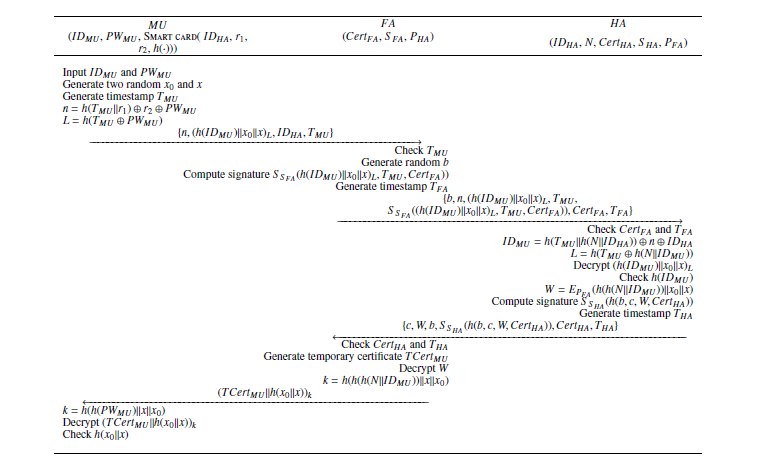
\includegraphics[width=1\textwidth]{1.png}
  \caption{First phase of Kang et al.'s scheme}\label{fig1}
\end{figure} \\
$MU's$ mobile device sends $MU$'s login message ${n,(h(ID_{MU})||x_{0}||x_{L},ID_{HA},T_{MU})}$ to $FA$, where $T_{MU}$ is a current timestamp.
  \item $FA\rightarrow HA$: ${b,n,(h(ID_{MU})||x_{0}||x)_{L},T_{MU},S_{S_{FA}}((h(ID_{MU})||x_{0}||x_{L},T_{MU},Cert_{FA})),Cert_{FA},T_{FA}}$ $FA$ checks the validity of $T_{MU}$. If it is valid, then FA chooses secret random number b. FA then sends $b$, the $MU$'s login message containing ${n,(h(ID_{MU})||x_{0}||x_{L},ID_{HA},T_{MU})}$, a cerificate $Cert_{FA}$, timestamp $T_{FA}$, and the corresponding signature on the login message by using $FA$'s private key $S_{FA}$ to $HA$.
  \item $HA\rightarrow HA:$ ${c,W,b,S_{S_{HA}}(h(b,c,W,Cert_{HA}),Cert_{HA},T_{HA})}$
      $HA$ checks the validity of certificate $Cert_{FA}$ and timestamp $T_{FA}$. If they are valid, then $HA$ computes $MU's$ real identity $ID_{MU}$ as follows.
    \begin{equation}
    ID_{MU}=h(T_{MU}\|h(N||ID_{HA}))\oplus n\oplus ID_{HA}
    \end{equation}
    HA computes $L = h(T_{MU}\oplus h(N||ID_{MU}))$ with his/her secret $N$ and decrypts$(h(ID_{MU})||x_{0}||x)_{L}$. Then,$HA$ verifies if $MU$ is a legal user by checking $h(ID_{MU})=h(ID_{MU})'s$, where $h(ID_{MU})$ is computed with $ID_{MU}$ on the login message and $h(ID_{MU})'$ of the decrypting result ${h(ID_{MU})'||x'_{0}||x'}$. If so, then HA computes $W = E_{P_{FA}}(h(h(N||ID_{MU})||x_{0}||x))$ and generates its signature using his/her private key $S_{HA}$. Then, HA sends random number $c$, $W$, the certificate of $HA$, $Cert_{HA}$, current timestamp $T_{HA}$ and signaure $S_{S_{HA}}(h(b,c,W,Cert_{HA}))$ to FA.
  \item $FA\rightarrow MU:$ $(TCert_{MU}||h(x_{0}||x))_{k}$ $FA$ checks whether of not the certificate $Cert_{HA}$ and timestamp $T_{HA}$ are valid. If They are valid, then $FA$ issues the temporary certificate $TCert_{MU}$, which includes a timestamp and other information to $MU$. To obtain $(h(h(N||ID_{MU}))||x_{0}||x)$, $FA$ decrypts $W$ with the secret key corresponding to $P_{FA}$. To establish session key $k_{i}$ for $i$-th session, $FA$ first saves $(TCert_{MU},h(PW_{MU},x_{0}))$. $FA$ encrypts $(TCert_{MU}||h(x_{0}||x))$ with session key $k$ and gives $(TCert_{MU}||h(x_{0}||x))_{k}$ to $MU$. Here, the session key is computed as follows.
      \begin{equation}
    \begin{aligned}
    k&=h(h(h(h(N\|ID_{MU}))\|x\|x_0)\\
    &=h(h(PW_{MU}))\|x\|x_0
    \end{aligned}
    \end{equation}
  \item $MU$ computes $k$ and obtains $TCert_{MU}$. $MU$ also authenticates $FA$ by computing $h(x_{0}||x)$ with the decrypted $h(x_{0}||x)$. Therefore, $MU$ can be sure that it is communicating with a legal $FA$.
\end{enumerate}




\subsection{Second Phase}
When MU visits FA at the i-th session, MU sends the following login message to FA.
\begin{enumerate}
\item
MU$\rightarrow$FA:$TCert_{MU},(x_{i}||TCert_{MU}||Other Information)_{k_{i}}$ The new $i$-th key $k_{i}$ can be derived from the unexpired previous secret value $x_{i-1}$ and the fixed secret value $x$ as
\begin{equation}
k_i=h(h(h(h(N\|ID_{MU}))\|x\|x_{i-1}
\end{equation}
where $i= 1,\ldots,n.$
\item
Upon receiving a login message from $MU, FA$ decrypts($x_{i}||TCert_{MU}||OtherInformation)_{k_{i}}$ with $k_{i}$ and newly saves($TCert_{MU},h(PW_{MU}),x_{i}$) for the next communication.
\end{enumerate}

\section{Anonymity Problem of Kang et al.s Scheme}
Kang et al. \cite{ZYan122} improved Wu et al.'s scheme\cite{Lohr10} and Weiet al's scheme \cite{Ateniese11} to provide anonymity. Based on thegeneral interest of mobile users, user anonymity shouldbe kept from any eavesdroppers including the foreign agents \cite{Barsoum11}. However, Kang et al.'s scheme still cannot provide anonymity. The main reason is that HA always computes ri for each MU withlthe same secret key N. The detailed anonymity broken attack scenario is as follows.
\begin{enumerate}
  \item Any legal user MU can directly obtain $h(N||ID_{HA})$
from $r_{i}$ in his/her smart card because $r_{i} = h(N||ID_{HA})$
from the Eq.\cite{Zhang10}.
  \item The legal user MU can collect the messages $\{n',h(ID'_{MU})||x'_{0}||x')_{L'},ID_{HA},T'_{MU}\}$ sent from any other legal mobile user MU' to FA at step \cite{Li10} in the first phase (see Fif,1). From the Eqs.\cite{Li10,Zhang10,Lohr10,WangWRL10},we can see that $n'$ is equal to $h(T'_{MU}||r_{1})\oplus ID_{HA} \oplus ID'_{MU}$ as follows.

\begin{equation}
\begin{aligned}
n'=&h(T'_{MU}\|r_{1}\oplus PW'_{MU}\\
  =&h(T'_{MU}\|h(N\|ID'_{MU})\oplus ID_{HA}\\
   &  \oplus ID'_{MU}\oplus PW'_{MU} \\
  =&h(T'_{MU}\|r_{1})\oplus h(N\|ID'_{MU}\oplus ID_{HA})\\
   &  \oplus ID'_{MU}\oplus h(N\|ID'_{MU})\\
  =& h(T'_{MU}\|r_{1})\oplus ID_{HA}\oplus ID_{MU}
\end{aligned}
\end{equation}
  \item With obtained $r_{1} = h(N||ID_{HA}) $and collexted messages $\{n',ID_{HA},T'{MU}\}$, $MU$ can get the real identity $ID'_{MU}$ of the other mobile user MU' as HA does at step \cite{Lohr10} in the first phase as follows.
\begin{equation}
\begin{aligned}
ID'_{MU} =& n'\oplus(T'_{MU}\|r_{1})\\
         =& h(T'_{MU}\|r_{1})\oplus ID_{HA}\oplus ID'_{MU}\\
          & \oplus ID_{HA}\oplus h(T'_{MU}\|r_{1})\\
         =& ID'_{MU}
\end{aligned}
\end{equation}
\end{enumerate}
As a result, legal mobile user MU's anonymity cannot be preserved in Kang et al.'s scheme.
\section{Conclusions}
This letter demonstrated that recently pubished wireless authentication scheme by Kang et al's scheme did not solved the problem of user anonymity that was pointed out Zeng et al.\cite{WangWRL10} and Lee al.\cite{Barsoum11}.
\section*{Acknowledgements}
This research was supported by Basic Science Reseatch Program through the National Research Foundation of Korea(NRF) funded by the Ministry of Education, Science and Technology(No. 2010-0010106) and partially supported by the MKE(The Ministry) of Knowledge Economy),Korea under the ITRC(Information Technology Research Center) support program (NIPA-2012-H0301-12-2004) supervised by the NIPA (National IT Industry Promotion Agency).
\begin{thebibliography}{00}
\bibitem{Li10}
L. Ming, Y. Shucheng, R. Kui, and L. Wenjing, Securing Personal Health Records in Cloud Computing: Patient-Centric and Fine-Grained
Data Access Control in Multi-owner Settings, in: Processing of SecureComm 2010, LNICST 50, pp. 89-106, 2010.

\bibitem{Zhang10}
R. Zhang, and L. Liu, Security Models and Requirements for Healthcare Application Clouds, in: Processing of  Cloud 2010, pp. 268-275, 2010.

\bibitem{Lohr10}
H. Lohr, A.-R. Sadeghi, and M. Winandy, Securing the e-health cloud, in: Processing of  IHI 2010, pp. 220-229, 2010.

\bibitem{WangWRL10}
C. Wang, Q. Wang, K. Ren, W. Lou, Privacy-preserving public auditing for data storage security in cloud computing, in: Processing of IEEE INFOCOM 2010, San Diego, CA, 14-19 March, 2010, pp. 525-533.

\bibitem{Barsoum11}
A. F. Barsoum, and M. A. Hasan, On Verifying Dynamic Multiple Data Copies over Cloud Servers, Cryptology ePrint Archive: Report 2011/447, https://eprint.iacr.org/2011/447.


\bibitem{Ateniese11}
G. Ateniese, R. C. Burns, R. Curtmola, J. Herring, L. Kissner, Z.N.J. Peterson, D. Song,  Remote data checking using provable data possession, ACM Trans. Inf. Syst. Security, 14 (1) (2011) 12.

\bibitem{ZYan122}
Y. Zhu, H. Hu, G. J. Ahn, M.Yu, Cooperative provable data possession for integrity verification in multicloud storage, IEEE Trans. Parallel Distrib. Syst., 23 (12) (2012) 2231-2244.


\bibitem{Juels07}
A. Juels, B. S. Kaliski, PORs: proofs of retrievability for large files, in: Proceeding of ACM CCS'07, Alexandria, Virginia, USA, Oct.29-Nov.2, 2007, pp. 584-597.

\bibitem{ShaWaters12}
H. Shacham, B. Waters, Compact proofs of retrievability, Journal of Cryptology, 26 (3) (2013) 442-483.


%\bibitem{WangWRLL11}
%Q. Wang, C. Wang, K. Ren, W. Lou, J. Li, Enabling public audibility and data
%dynamics for storage security in cloud computing, IEEE Trans. Parallel Distrib. Syst., 22 (2011) 847-859.
%
%
%\bibitem{WangChowWangRenLou}
%C. Wang, S.S. Chow, Q. Wang, K. Ren, W. Lou, Privacy-preserving public
%auditing for secure cloud storage, IEEE Transactions on Computers, 62 (2013) 362-375.
%
%\bibitem{bing13}
%J. Ni, Y. Yu, Y. Mu, Q. Xia, On the security of an efficient dynamic auditing protocol in cloud storage. IEEE Transactions on Parallel and Distributed Systems. (2013) Doi: 10.1109/TPDS.2013.199.
%
%\bibitem{Yu20144}
%Y. Yu, L. Niu, G. Yang, Y. Mu, and W. Susilo, On the security of auditing mechanism for secure cloud storage, Further Generation Computer Systems, 30 (127-132), 2014.
%
%\bibitem{fan2013}
%X. Fan, G. Yang, Y. Mu, Y. Yu, On Indistinguishability in Remote Data Integrity Checking, The Computer Journal, doi: 10.1093/comjnl/bxt13, 2013.
%
%\bibitem{Chen13}
%L. Chen, S. Zhou, X. Huang, L. Xu, Data dynamics for remote data possession checking in cloud storage, Computers and Electrical Engineering, 39, pp. 2413-2424, 2014.
%
%\bibitem{Yu2014}
%Y. Yu, J. Ni, H. Wang, C. Xu, Improved security of a dynamic remote data possession checking protocol for cloud storage, Expert System with Applications, doi: http:// dx.doi.org/ 10.1016/j.eswa. 2014.06.027, 2014.
%
%\bibitem{Huaqun14}
%H. Wang, Q. Wu, B. Qin, and D.-F. Josep, FRR: Fair remote retrieval of outsourced private medical records in
%electronic health networks, Journal of Biomedical Informatics, http://dx.doi.org/10.1016/j.jbi.2014.02.008, 2014.
%\bibitem{boneh2001}
%D. Boneh, M.K. Franklin, Identity-based encryption from the weil pairing, in: Processing of CRYPTO 2001, Santa Barbara, California, USA, 2001, pp. 213-229.

%\bibitem{bls2001}
%D, Boneh, B, Lynn, H, Shacham, Short signatures from the weil pairing, in: Processing of ASIACRYPT 2001, Gold Coast, Australia, 2001, pp. 514-532.

\end{thebibliography}
\end{document}
